\chapter{Theory}

\section{Bias point and class operation}
The bias point, or working point, of an amplifier determines which class the amplifier is, which in turn tells us something about the amplifiers efficiency, linearity and quiescent current. There is a wide variety of classes, the most common being class A, AB, B and C. 
Class A amplifiers have the highest quiescent current, the best linearity and the lowest efficiency (maximum theoretical efficiency of 50\% ). 
Class B amplifiers have no quiescent current, maximum theoretical efficiency of 78\% , but only conducts the positive half-period of a signal. 
Class AB is a hybrid between class A and B, sacrificing some of the efficiency of the class B amplifier, but gaining some of the linearity of the class A. 
Class C amplifiers are the most efficient of the four, having a maximum theoretical efficiency of almost 90\% . But they conduct for less than 50\%  of the signal cycle, typically they only conduct for a third of the cycle or less.
If the input signal of the amplifier is sufficiently small, one can bias the amplifier as an AB class, thus reducing quiescent current while still have class A operation in terms of linearity.

Once a class has been chosen, the bias point can be determined by examining the I-V characteristics of the transistor. By drawing a loadline going from the drain-source voltage on the X axis, to the drain saturation current on the Y axis, we get a linear line crossing the different gate-source voltage curves. See figure~\ref{fig:fig_Load_line}. By choosing a bias point along this linear curve, we can predict both quiescent current and voltage. The bias point for a class A amplifier will approximately be at Vds/2. The closer you move the bias point towards the maximum Vds voltage, the lower the class you get. This is because the loadline represents the current through and voltage across the transistors equivalent resistor.

\begin{figure}[H]
	  \centering
	  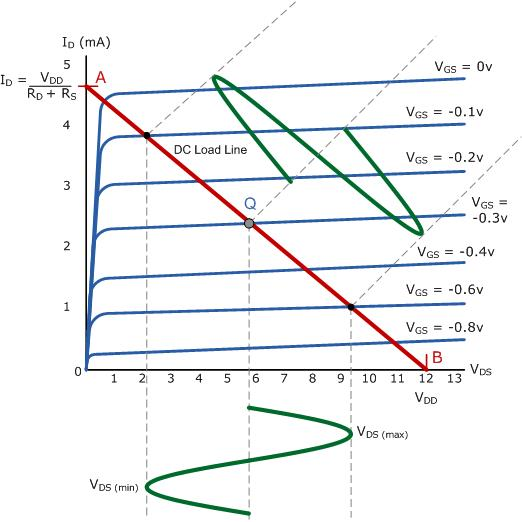
\includegraphics[width=0.75\textwidth]{img/Load_line_graphics}
	  \caption{Load line for class A amplifier}
	  \label{fig:fig_Load_line}
\end{figure}

\section{Efficiency}
There are several ways of expressing amplifier efficiency, the most common in the RF community being power added efficiency (PAE). PAE takes into account both the DC to RF power conversion, as well as the RF power delivered into the input of the device.

\begin{equation}
	PAE=\frac{P_{RFout}-P_{RFin}}{P_{DC}}=\frac{P_{RFout}-P_{RFin}}{V_{DC} \times I_{DC}} 
\end{equation}
\section{Linearity}

\section{S-parameters}

\section{Stability}

\section{Quarter wave transformation}

\section{Matching}

\section{Small signal vs large signal}

\section{Intermodulation distortion}
